% \onecolumn

% \section*{Overview of Appendix}

% This appendix provides supplementary materials for the main paper, including experimental protocol details, factor-pool export rules, ablation designs, and extended robustness/predictability results.

% \section{Further Related Work}
% \label{sec:appendix_related_work}

% \subsection{Automated Alpha Mining Before LLMs}

% Traditional alpha mining began with human-designed factor models and anomaly-based formulas. In automated settings, genetic programming and related evolutionary search became the earliest practical route for exploring large formula spaces. AutoAlpha improves search efficiency through hierarchical initialization, while AlphaEvolve extends the search object from formula trees to richer computation graphs \cite{zhang2020autoalpha,cui2021alphaevolve}. Reinforcement learning then reframed alpha discovery as a sequential decision problem. AlphaGen uses policy optimization to generate collaborative formulaic alpha sets, and AlphaForge introduces a generative-predictive architecture with dynamic factor combination \cite{yu2023alphagen,shi2025alphaforge}. These methods established the importance of large-scale search, but they still largely treat search as operating over syntax or operator composition rather than an explicit economic mechanism.

% \subsection{LLM-Based Alpha Mining}

% LLM-based alpha mining methods can be grouped by their primary search object. FAMA uses in-context factor examples and chain-of-experience reuse to generate compact factor sets, and admits a factor only if it improves pool-level utility \cite{li2024can}. AlphaAgent regularizes generation through originality, semantic consistency, and AST complexity control, then uses a downstream LightGBM combiner over validated factors \cite{tang2025alphaagent}. MCTS-Alpha maintains an alpha zoo, filters candidates by predictive quality and correlation, and selects top-\(k\) factors for downstream modeling \cite{shi2025navigating}. FactorEngine lets the LLM search over executable programs rather than closed-form expressions, and screens elites through a composite fitness score \cite{lin2026factorengine}.

% Several newer systems broaden the search object even further. QuantaAlpha evolves full mining trajectories through planning, mutation, and crossover, and evaluates all LLM-based methods with a unified downstream LightGBM protocol over roughly 150 validated factors \cite{quantaalpha2026}. Hubble emphasizes safe and reproducible generation: it evaluates guarded candidates in rounds, applies family-aware diversity constraints, and validates only the top selected factors on a held-out period \cite{shi2026hubble}. CogAlpha adopts code-level evolution with explicit parent, child, and elite pools, using multi-metric percentile gates to maintain quality \cite{cogalpha2025}. AlphaSAGE, in contrast, focuses on sampling a diverse high-reward alpha library through a structure-aware GFlowNet objective rather than a fixed-size final pool \cite{chen2025alphasage}. Across these methods, factor quality, factor-pool construction, and evaluation protocol are tightly coupled.

% \subsection{Agentic Search, Memory, and Self-Evolution}

% The broader agentic literature provides two additional lessons. First, finance-specific multi-agent systems such as RD-Agent and TradingAgents show that role specialization, staged workflows, and execution-grounded feedback can stabilize complex decision pipelines \cite{li2025r,xiao2024tradingagents}. Second, memory-centric systems such as FinMem and FinCon show that long-horizon financial reasoning benefits from retaining structured experience rather than relying on single-turn prompting \cite{yu2025finmem,yu2024fincon}. Beyond finance, AlphaEvolve and controlled self-evolution systems demonstrate how code agents can improve under evaluator-driven feedback \cite{novikov2025alphaevolve,hu2026controlled}. \method{} inherits these insights, but attaches memory and repair to structured semantic plans rather than to unrestricted trajectories.

% \subsection{Factor-Pool Selection Protocols}

% An experimentally consequential but often under-specified issue is how candidate factors are converted into the final evaluation pool. Existing papers follow at least three families of protocols. \textbf{Large-pool downstream combination} is exemplified by QuantaAlpha, where each LLM method contributes roughly 150 validated factors and the final comparison is made under a shared downstream LightGBM model \cite{quantaalpha2026}. \textbf{Elite-pool or top-\(k\) selection} appears in MCTS-Alpha and FactorEngine, which maintain an effective repository during search and export a smaller high-quality subset after correlation or fitness filtering \cite{shi2025navigating,lin2026factorengine}. \textbf{Dynamic or utility-based pool construction} appears in FAMA, AlphaForge, AlphaSAGE, and Hubble, where the emphasis is not a fixed \(K\), but whether a candidate improves utility, supports dynamic weighting, or preserves diversity at the family level \cite{li2024can,shi2025alphaforge,chen2025alphasage,shi2026hubble}. This distinction is especially relevant for \method{}, whose scorer acts on semantic plans before code generation, whereas all final claims must still be made through a transparent factor-pool protocol.




\section{Evaluation Details}
\label{sec:appendix_eval_details}

\subsection{Experimental Protocol}
\label{sec:appendix_exp_setup}

We use CSI300 as the stock universe and SH000300 as the benchmark index. The time span is split into training (Jan 1, 2016 -- Dec 31, 2020), validation (Jan 1, 2021 -- Dec 31, 2022), and testing (Jan 1, 2023 -- Dec 31, 2025). The main label is the 5-day forward return:
\begin{equation}
y_{i,t}=\frac{\mathrm{Ref}(\mathrm{close},-6)}{\mathrm{Ref}(\mathrm{close},-1)}-1.
\end{equation}
Factor selection, correlation filtering, and model selection are performed only on the training and validation windows. The 2023--2025 period is reserved for held-out reporting.

\subsection{Downstream Combiner for Factor Pools}

For methods that produce an explicit factor pool, the selected factors are combined by a LightGBM ranker. Given an exported factor pool \(\mathcal{F}=\{f_1,\ldots,f_K\}\), we construct
\begin{equation}
z_{i,t}=[f_1(i,t),\ldots,f_K(i,t)]
\end{equation}
for stock \(i\) on day \(t\). Missing values and infinite values are processed before training, invalid labels are removed, and both features and labels are normalized by cross-sectional rank normalization. LightGBM is trained on the training window, while early stopping and hyperparameter selection use the validation window before test evaluation. The factor-pool experiments use 500 boosting rounds, early stopping after 50 rounds without validation improvement, and a fixed hyperparameter configuration across the corresponding factor-pool runs.

\subsection{Predictive Metrics}

We follow the standard factor-evaluation convention used in Qlib-style alpha-mining papers and report both linear-correlation and rank-correlation metrics. For each test day \(t\), let \(\hat y_{i,t}\) be the model score, \(y_{i,t}\) the realized label, and \(\mathcal{U}_t\) the tradable cross-section after suspension, missing-label, and validity filters.

\textbf{Information Coefficient (IC).}
IC measures whether predicted scores are linearly aligned with realized cross-sectional returns:
\begin{equation}
\begin{aligned}
\mathrm{IC}_t
&=\mathrm{corr}_{i\in\mathcal{U}_t}(\hat y_{i,t},y_{i,t}),\\
\mathrm{IC}
&=\frac{1}{|\mathcal{T}_{\mathrm{test}}|}
  \sum_{t\in\mathcal{T}_{\mathrm{test}}}\mathrm{IC}_t .
\end{aligned}
\end{equation}

\textbf{IC Information Ratio (ICIR).}
\begin{equation}
\mathrm{ICIR}=\frac{\mathrm{mean}_{t}(\mathrm{IC}_t)}{\mathrm{std}_{t}(\mathrm{IC}_t)}.
\end{equation}

\textbf{Rank Information Coefficient (Rank IC).}
\begin{equation}
\begin{aligned}
\mathrm{RankIC}_t
&=\mathrm{corr}_{i\in\mathcal{U}_t}
  \bigl(\mathrm{rank}(\hat y_{i,t}),\mathrm{rank}(y_{i,t})\bigr),\\
\mathrm{RankIC}
&=\frac{1}{|\mathcal{T}_{\mathrm{test}}|}
  \sum_{t\in\mathcal{T}_{\mathrm{test}}}\mathrm{RankIC}_t .
\end{aligned}
\end{equation}

\textbf{Rank IC Information Ratio (Rank ICIR).}
\begin{equation}
\mathrm{RankICIR}=\frac{\mathrm{mean}_{t}(\mathrm{RankIC}_t)}{\mathrm{std}_{t}(\mathrm{RankIC}_t)}.
\end{equation}
Predictive metrics are computed on the held-out test/backtest window and do not include transaction costs. Days with too few tradable assets or degenerate prediction/label vectors are excluded.

\subsection{Trading Strategy}

Strategy-level evaluation uses Qlib's \texttt{TopkDropoutStrategy} with \texttt{topk=50} and \texttt{n\_drop=5}. On each rebalance date, stocks are ranked by \(\hat y_{i,t}\). The target portfolio holds the top 50 names with equal weights. To reduce turnover, existing holdings that remain sufficiently highly ranked are retained; at most five lowest-ranked current holdings are replaced by the highest-ranked non-held names. Rebalancing is daily. This Top50/Drop5 rule follows recent Qlib-based alpha-mining protocols and keeps the comparison focused on signal quality rather than portfolio optimization.

\subsection{Execution Assumptions and Costs}

Trades are executed at the \textbf{open price} on the trading day after signal generation (\texttt{deal\_price=open}). Transaction costs are modeled as a buying cost of 0.05\% and a selling cost of 0.15\%, with a minimum fee of 5 currency units per trade and a round-trip friction of approximately 0.20\%. Limit-up/limit-down filtering is enabled with \texttt{limit\_threshold=0.095}. Untradable names are skipped for new purchases, while existing holdings are handled according to Qlib exchange rules.

\subsection{Portfolio Metrics}

Predictive metrics measure ranking quality but not tradability. We therefore report portfolio-level metrics under the Top50/Drop5 strategy. Let \(r^{\mathrm{port}}_t\) be the portfolio return, \(r^{\mathrm{bench}}_t\) the CSI300 benchmark return, and \(c_t\) the transaction-cost term. The daily excess return is defined as
\begin{equation}
e_t = r^{\mathrm{port}}_t - r^{\mathrm{bench}}_t - c_t,
\end{equation}
where the benchmark is SH000300. All portfolio metrics below are computed from \(\{e_t\}\) with \(N=252\) trading days per year.

\textbf{Annualized Excess Return (AER).}
\begin{equation}
\mathrm{AER}=\left(\prod_{t=1}^{T}(1+e_t)\right)^{252/T}-1.
\end{equation}
AER is therefore the annualized benchmark-relative excess return after transaction costs, rather than the annualized raw portfolio return.

\textbf{Information Ratio (IR).}
\begin{equation}
\mathrm{IR}=\frac{\mathrm{mean}_t(e_t)}{\mathrm{std}_t(e_t)}\sqrt{252}.
\end{equation}
Because the excess return is defined relative to CSI300 rather than a risk-free rate, IR measures benchmark-relative risk-adjusted performance.

\textbf{Maximum Drawdown (MDD).}
MDD is computed on the cumulative excess-return curve induced by \(\{e_t\}\):
\begin{equation}
\mathrm{MDD}=\max_{t\leq T}\left(1-\frac{C_t}{\max_{s\leq t}C_s}\right),
\quad
C_t=\prod_{s=1}^{t}(1+e_s).
\end{equation}

% \section{Additional Ablation Details}
% \label{sec:appendix_ablation}

% \subsection{Schema Grammar Ablation}

% The schema ablation is a leave-one-component-out experiment over the five semantic fields \(E, C, Q, D, O\). Removing a component means replacing it with a null field while preserving the rest of the plan and the same execution contract. This is stricter than comparing only against a free-form baseline because it identifies which semantic field carries predictive or regularizing value.

% \begin{table}[h]
% \centering
% \caption{Detailed schema-ablation design.}
% \label{tab:appendix_schema_ablation_design}
% \begin{tabular}{p{0.22\textwidth} p{0.70\textwidth}}
% \toprule
% \textbf{Variant} & \textbf{Interpretation} \\
% \midrule
% w/o Event & Tests whether explicit market phenomena are the primary carriers of signal quality. \\
% w/o Context & Tests whether regime conditioning materially improves implementation and generalization. \\
% w/o Qualities & Tests whether reliability filters are needed beyond the raw event-context pair. \\
% w/o Direction & Tests whether semantic interpretation of the event materially affects downstream utility. \\
% w/o Output & Tests whether explicit signal-emission type is necessary for robust realization. \\
% Free-form Prompting & Removes the schema grammar entirely and reverts to unconstrained natural-language generation. \\
% \bottomrule
% \end{tabular}
% \end{table}

% \subsection{Scheduler Ablation}

% The scheduler ablation compares adaptive mixing against fixed or degenerate strategies. The main hyperparameters are: score temperature \(\tau\), exploration quota \(\alpha\), and mutation quota \(\beta\). These parameters determine whether the selector collapses to scorer-driven exploitation, coverage-driven exploration, or a stable hybrid regime. The corresponding sensitivity curves are reserved for the final experimental figure in the main paper.

% \subsection{Predictability of Schema Space}

% The scorer is evaluated as a semantic ranking model under three settings:
% \begin{itemize}
%     \item \textbf{In-round random holdout}: random plans from the same round are hidden during scorer fitting.
%     \item \textbf{Future-round holdout}: the scorer is fit on early rounds and tested on later rounds.
%     \item \textbf{Cross-topic holdout}: certain semantic topic families are excluded from training and used only for evaluation.
% \end{itemize}
% The relevant metrics are Spearman rank correlation, top-decile precision, NDCG@K, and calibration gap. This experiment directly tests whether semantic structure is predictable before implementation.

\section{Additional Ablation Details}
\label{sec:appendix_ablation}

\subsection{Formal Schema Notation}
\label{sec:appendix_schema_notation}

The semantic plan space is written as
\[
  \mathcal{P} = \mathcal{E} \times \mathcal{C} \times 2^{\mathcal{Q}}
                \times \mathcal{D} \times \mathcal{O}.
\]
Here \(\mathcal{P}\) denotes the set of all candidate plans. The five component
sets correspond to \emph{Event} choices \(\mathcal{E}\), \emph{Context} choices
\(\mathcal{C}\), \emph{Quality} choices \(\mathcal{Q}\), \emph{Direction}
choices \(\mathcal{D}\), and \emph{Output} choices \(\mathcal{O}\). We use
\(2^{\mathcal{Q}}\) for qualities because a plan may include multiple
confirmation or filtering conditions, whereas the other fields usually select
one primary option.

Thus, a plan can be written as \(p=(e,c,Q,d,o)\), where \(e\in\mathcal{E}\),
\(c\in\mathcal{C}\), \(Q\subseteq\mathcal{Q}\), \(d\in\mathcal{D}\), and
\(o\in\mathcal{O}\). Its canonical key is
\[
  \operatorname{key}(p)=e\mid c\mid q_1\mid\cdots\mid q_m\mid d\mid o,
\]
which supports deduplication, coverage tracking, mutation, and surrogate
scoring.



\subsection{Factor-Pool Export and Artifact Scope}

For auditability, we maintain an export package for the +Fundamental-schema \method{} factor pool reported in Table~\ref{tab:main_eval}. The current package contains 150 factor source files, consisting of 60 EBS reward factors and 90 factors inherited from a previous top-150 pool after correlation-aware selection; the latter subset includes 68 price-volume factors and 22 fundamental factors. Each exported factor records its selected period, candidate periods, direction adjustment, source group, and source-code mapping. The export also includes selection manifests, period-audit tables, saved Qlib configuration, metric snapshots, and plot data for regenerating reported curves.

\begin{table}[t]
\centering
\caption{Summary of the exported factor-pool artifact.}
\label{tab:appendix_export_scope}
\small
\begin{tabularx}{\columnwidth}{lX}
\toprule
\textbf{Item} & \textbf{Value} \\
\midrule
Exported factor sources & 150 \\
EBS factors & 60 \\
Previous-pool factors & 90 \\
Most common selected periods & 20, 80, 60 \\
Included artifacts & source, manifest, period audit, config, metrics, curves \\
Excluded artifacts & raw market data, labels, factor-value parquet files \\
\bottomrule
\end{tabularx}
\end{table}

This artifact supports source inspection, configuration review, period auditing, and figure regeneration from saved curves. It is not intended as a complete raw-data reproduction package, since exact reruns also depend on the original data preprocessing and factor materialization environment.

\subsection{Final Factor-Pool Selection}

The final modeling pool is selected from the validated factor pool by a rank-and-filter rule. Let \(\mathcal{V}\) denote the set of valid candidate factors with available Rank IC scores. Candidates are first sorted in descending order by Rank IC (RIC). We then scan this ordered list greedily and add a candidate \(f\) to the selected pool \(\mathcal{S}\) only if
\begin{equation}
\max_{g\in\mathcal{S}} |\mathrm{corr}(f,g)| < 0.7,
\end{equation}
where the correlation is computed from factor values on the pool-selection window. This rule prioritizes individually strong factors while controlling redundancy in the exported pool. The reported export contains 150 factors: 60 newly selected EBS factors and 90 factors inherited from the previous top-150 pool after the same correlation-aware selection procedure.


\subsection{Schema Grammar Ablation}

The schema ablation is a leave-one-component-out experiment over the five semantic fields \(E, C, Q, D, O\). We sample 100 high-reward full schema plans and construct five blind variants for each plan by removing one field at a time. The implementation agent receives only the visible fields and is not told which component was removed. This yields 500 implementation tasks, of which 466 pass the full validity and evaluation pipeline. The primary metric is mean absolute Rank IC, because this experiment measures whether a generated factor contains ranking information regardless of whether the profitable direction is positive or negative.

\begin{table}[t]
\centering
\caption{Detailed schema-grammar leave-one-out results. Full is the source full-plan reference used to construct the ablation tasks.}
\label{tab:appendix_schema_ablation_design}
\setlength\tabcolsep{3pt}
\small
\resizebox{\columnwidth}{!}{%
\begin{tabular}{lccccc}
\toprule
\textbf{Variant} & \textbf{Missing Field} & \textbf{Valid} & \(\mathbf{|RankIC|}\uparrow\) & \textbf{Rel. (\%)} & \textbf{Reward} \\
\midrule
\method{} (Full source) & -- & 100/100 & 0.0185 & 100.0 & 4.174 \\
w/o Event & Event & 93/100 & 0.0147 & 78.9 & 2.199 \\
w/o Context & Context & 94/100 & 0.0131 & 69.4 & 2.249 \\
w/o Qualities & Qualities & 95/100 & 0.0134 & 72.9 & 2.483 \\
w/o Direction & Direction & 88/100 & 0.0134 & 71.7 & 2.219 \\
w/o Output & Output & 96/100 & 0.0141 & 75.1 & 2.310 \\
\bottomrule
\end{tabular}
}
\end{table}

The full reference is not reimplemented under the blind ablation prompt; it is read from the source full-plan runs used to build the 100-plan task set. We therefore use this experiment as a component-level diagnostic rather than as a final portfolio-level comparison. A complete paired subset in which all five ablated variants are valid contains 71 source plans and yields the same qualitative ordering: every leave-one-out variant remains below the full source reference.

Figure~\ref{fig:schema_leave_one_out} visualizes the same comparison in the main paper. Every field removal reduces retained signal strength, while most variants still maintain high implementation validity. The degradation is therefore not only an execution failure effect, but also reflects weaker schema semantics.

\subsection{Code-Agent Backend Robustness}
\label{sec:appendix_code_agent_robustness}

This experiment isolates the effect of the implementation backend. We fix the same 100 schema plans and ask six code agents to realize them. Pass@1 records first-attempt success; failed cases receive at most one retry/repair when available. A run is counted as successful only when the generated factor passes evaluation and receives a valid reward. Signal quality is measured by mean \(|\mathrm{RankIC}|\) over final successful factors.

\begin{table}[t]
\centering
\caption{Repair-aware code-agent backend robustness on the same 100 schema plans. Kimi is reported under pass@1 only because retry was not available in this export.}
\label{tab:appendix_code_agent_robustness}
\setlength\tabcolsep{3.4pt}
\small
\resizebox{\columnwidth}{!}{%
\begin{tabular}{lccccc}
\toprule
\textbf{Backend} & \textbf{Pass@1} & \textbf{Repair} & \textbf{Final} & \(\mathbf{|RankIC|}\uparrow\) & \textbf{RankIC} \\
\midrule
GPT-5.4 & 97/100 & 2 & 99/100 & 0.0116 & 0.0040 \\
GPT-5.4-mini & 81/100 & 10 & 91/100 & 0.0129 & 0.0073 \\
Kimi-K2.7-Code & 82/100 & 0 & 82/100 & 0.0138 & 0.0075 \\
DeepSeek-V4-Flash & 63/100 & 30 & 93/100 & 0.0168 & 0.0121 \\
Qwen3.6-Flash & 49/100 & 40 & 89/100 & 0.0161 & 0.0115 \\
GLM-5.2 & 75/100 & 22 & 97/100 & 0.0145 & 0.0109 \\
\bottomrule
\end{tabular}
}
\end{table}

The corresponding visualization is reported in Figure~\ref{fig:code_agent_model_invariance} in the main paper. The results separate execution reliability from factor quality. Retry mainly improves completion rates for lower Pass@1 backends, while successful factors from different backends remain in a comparable signal range. This supports the view that the schema provides transferable implementation intent rather than relying on a single agent backend.

\subsection{Predictability of Schema Space}
\label{sec:appendix_schema_predictability}

The predictability experiment evaluates whether reward can be inferred from the discrete schema representation alone. The dataset contains 12,126 valid plan--reward pairs and 11,295 unique schema keys. We use an 80/20 split, resulting in 2,430 held-out test examples. The target reward follows the historical factor-mining reward used in the search logs:
\begin{equation}
r=\frac{10\mathrm{IC}+\mathrm{ICIR}+10\mathrm{RankIC}+\mathrm{RankICIR}}{4}.
\end{equation}
The feature construction intentionally excludes schema text embeddings, TF--IDF features, generated code, factor values, and backtest trajectories. The two main feature sets are: (i) single-schema indicators with category/scope counts; and (ii) schema-pair features with pairwise schema and category-family-scope interactions. The mean baseline predicts a constant reward, while the shuffled-reward control preserves the feature matrix and model class but randomly permutes reward labels.

\begin{table}[t]
\centering
\caption{Full predictability results for schema-space reward prediction. Top10\% lift is measured against random selection.}
\label{tab:appendix_schema_predictability_full}
\setlength\tabcolsep{3pt}
\small
\resizebox{\columnwidth}{!}{%
\begin{tabular}{llcccc}
\toprule
\textbf{Feature Set} & \textbf{Model} & \(\rho_S\) & \(\rho_P\) & \textbf{RMSE$\downarrow$} & \textbf{Top10\% Lift} \\
\midrule
Mean baseline & Mean & 0.000 & 0.000 & 0.0908 & 1.000 \\
Single schema & Ridge & 0.212 & 0.214 & 0.0892 & 1.413 \\
Single schema & ElasticNet & 0.214 & 0.217 & 0.0888 & 1.381 \\
Single schema & LGBM & 0.237 & 0.245 & 0.0884 & 1.506 \\
Single schema & MLP & 0.121 & 0.123 & 0.0963 & 1.295 \\
Schema + pair interaction & LGBM & \textbf{0.239} & \textbf{0.250} & \textbf{0.0884} & \textbf{1.519} \\
Schema + pair interaction & MLP & 0.204 & 0.201 & 0.0903 & 1.273 \\
Shuffled reward & LGBM & 0.029 & 0.021 & 0.0917 & 0.946 \\
\bottomrule
\end{tabular}
}
\end{table}

The shuffled-reward control remains near random, supporting that the observed predictability reflects a genuine schema--reward relationship rather than feature dimensionality alone.

\begin{figure}[t]
    \centering
    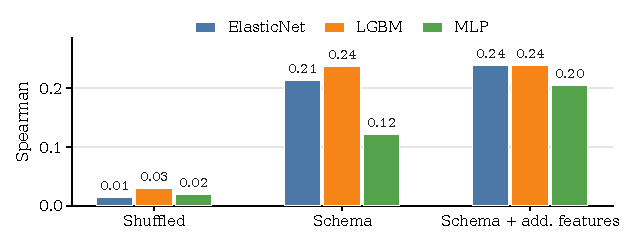
\includegraphics[width=\columnwidth]{figures/compact_learnability_spearman.pdf}
    \caption{Reward predictability from structured schema features.}
    \label{fig:schema_predictability}
\end{figure}

Figure~\ref{fig:schema_predictability} visualizes the same control logic:
schema features yield nontrivial ranking and top-decile enrichment, pair
interactions add a small gain, and shuffled rewards collapse toward random
selection.
